\documentclass[main.tex]{subfiles}

\begin{document}

	\begingroup

	\renewcommand{\cleardoublepage}{}

	\renewcommand{\clearpage}{}

	\chapter{Architecture Overview}
	\chapterauthor{Torge Olliges,\\ Marc Stelter}
		In this chapter the architecture and interaction between the different components will be summarized and explained.
		In order to cope with the previously introduced challenges, the following five expert groups have been formed:

		\begin{itemize}
			\item Navigation: Movement and localization
			\item Perception: Recognition of objects and classification
			\item Knowledge: Storage and providing access to information about the world state and object positions
			\item NLP: Speech processing and generation
			\item Manipulation: Interaction with objects within the world
			\item Planning: Decision making, execution of plans and error handling
		\end{itemize}
		
		\section{Basic Architecture}
		
		\begin{figure}[h]
			\centering
			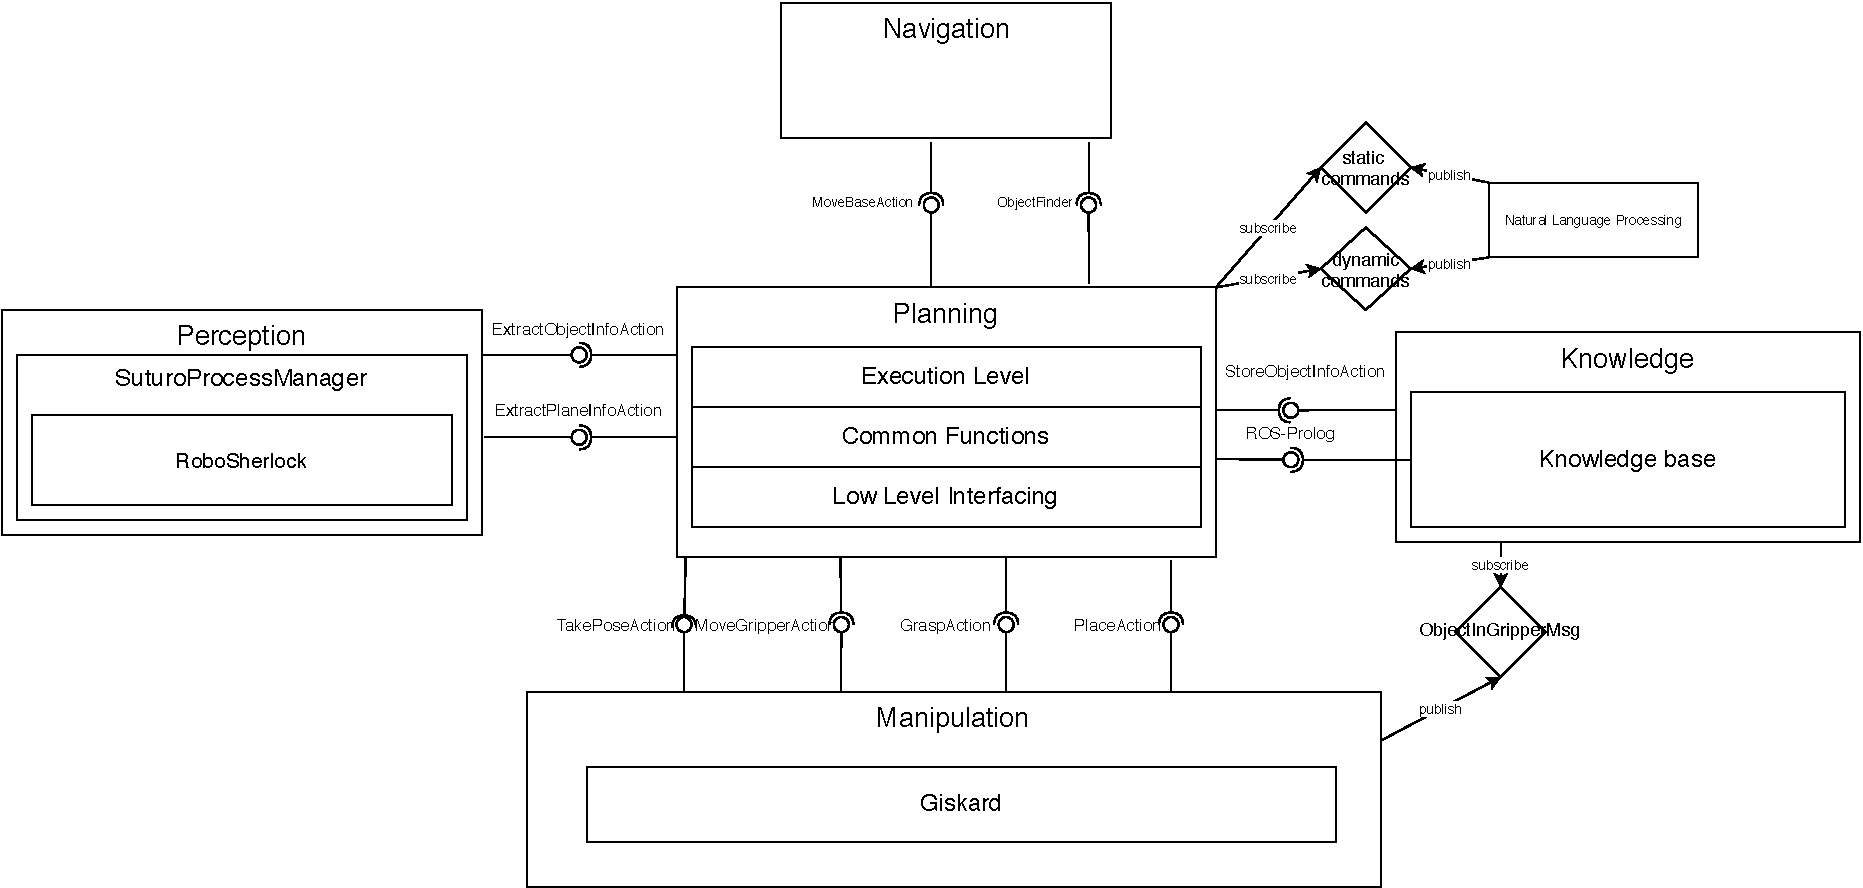
\includegraphics[width=1.0\textwidth]{pictures/diagramms/overview.pdf}
			\caption{Architecture overview}
			\label{architecture}
		\end{figure}
		

			In the diagram \(\ref{architecture}\) the components each group was responsible for are visualized. The Perception component consists mainly of the \textit{SuturoProcessManager} module which implements a process manager to execute the \textit{RoboSherlock} pipeline. The \textit{RoboSherlock} pipeline then handles the classification and annotation. The results are collected and converted by the \textit{SuturoProcessManager}.  The Knowledge component consists of the Knowledge base, which is a wrapped information storage (database) for the HSR. It handles position data as well as some logic for goal position determination. The Manipulation component is responsible for gripper, head, body movement and grasp, place operations. For this Manipulation is using \textit{Giskard}. The Navigation component is only used for moving the HSR and for collision avoidance during movement and uses the basic movement interface of the HSR. The Planning component uses \textit{Cram} to implement multi layered plans for executing the tasks. It is split into different hierarchical levels; cleanup \ref{clean} and grocery \ref{grocery} being on the highest level (execution level). These packages contain plans which call functions from the mid level (common functions) \ref{comf}. The lowest level used for communication with other groups low level interfacing \ref{llif}.
			
			\begin{itemize}
				\item{\textbf{Cram}} \\
					 \textit{Cram} (Cognitive Robot Abstract Machine) is a software toolbox for the design, the implementation, and the deployment of cognition-enabled autonomous robots performing everyday manipulation activities.
				\item{\textbf{Giskard}} \\
					\textit{Giskard} is a  framework for constraint based motion planning and execution.
				\item{\textbf{Julius}} \\
					\textit{Julius} is a continuous speech recognition software. It is capable of recognizing spoken sentence as-live. Julius' main strength is the fact that it works on dictionaries. Dictionaries are a simple way for developers to adapt Julius to only recognize domain-specific sentences. Julius is not specifically created for ROS, but Toyota created a wrapper to allow the output of Julius to be published in ROS.
				\item{\textbf{KnowRob}} \\
				    \textit{KnowRob} is a framework created to combine different knowledge sources (such as knowledge about and provided by the robot, common sense, research etc.) and provide reasoning methods to work with them. 
				\item{\textbf{RoboSherlock}} \\
					\textit{RoboSherlock} is a common framework for cognitive perception, based on the principle of unstructured information management (UIM).
				\item{\textbf{Caffe}} \\
					\textit{Caffe} is a deep learning framework made with expression, speed, and modularity in mind. It is developed by Berkeley AI Research (BAIR) and by community contributors.
			\end{itemize}

		\section{Interfaces (noch in arbeit)}
		
		\begin{figure}[H]
			\centering
			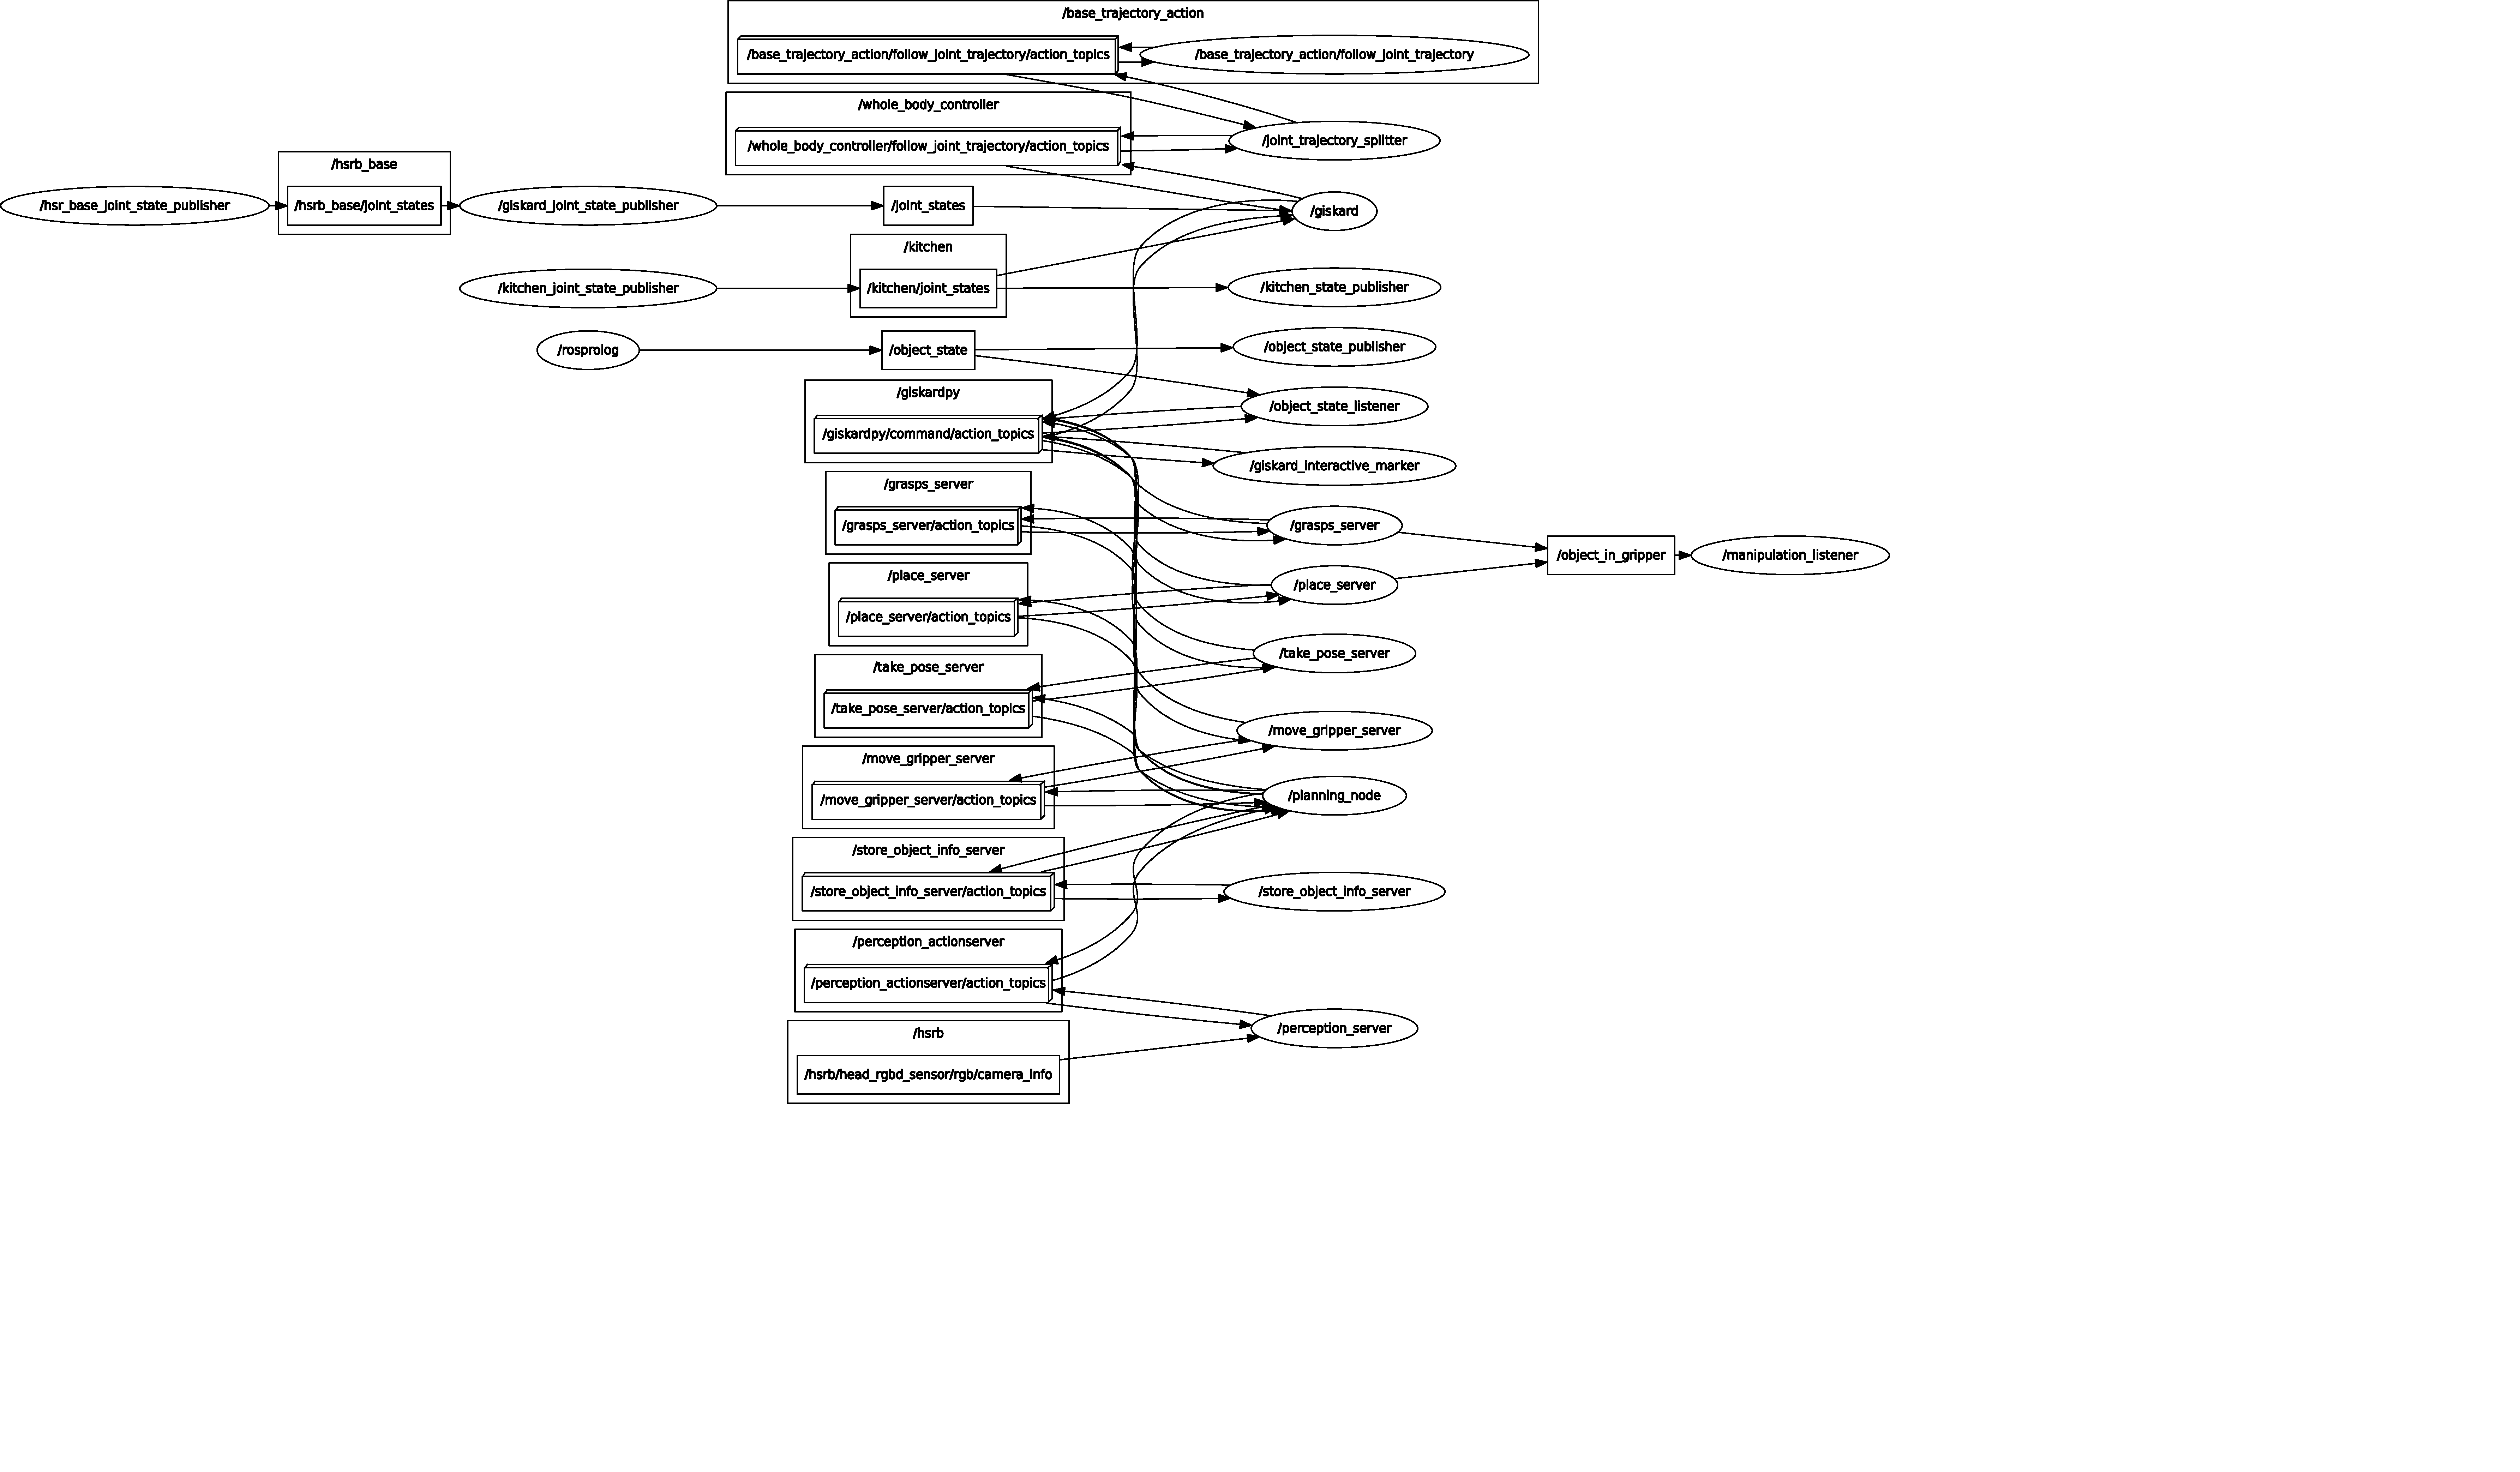
\includegraphics[width=1.0\textwidth]{pictures/diagramms/rosgraph}
			\caption{Interfaces}
			\label{interfaces}
		\end{figure}

		In figure \ref{interfaces} the action servers and some other communication can be seen. As the main node is the \textit{planning\_node} which requests actions from other servers like the \textit{place\_server} it is involved in all out communication. The sequence in which these calls are made will be explained in detail in chapter \ref{grocery-sequence} Storing Groceries Task Overview and chapter \ref{cleanup-sequence} Clean Up Task Overview.

		\subsection{Actionservers vs Topics}

		For our interfaces shown in \ref{interfaces} we chose to mainly use actionservers becasue they provide a simple synchronized form of communication where we can perform a task and then evaluate possible reactions to the new circumstances. This would not have been possible if we mainly used listener/subscriber structures with topic communication because that model would only provide assynchron communication where we can not be sure if the message were received and what the outcome of the requested action was.

		\subsection{Messages}


		
	  		 

	\endgroup

\end{document}
